\documentclass[11pt]{article}

\usepackage{graphicx}
\usepackage{wrapfig}
\usepackage{url}
\usepackage{wrapfig}
\usepackage{color}
\usepackage{marvosym}
\usepackage{enumerate}
\usepackage{subfigure}
\usepackage{tikz}
\usepackage{amsmath}
\usepackage{amssymb}
\usepackage{hyperref}
\usepackage{epstopdf}

\def\ci{\perp\!\!\!\perp}

\oddsidemargin 0mm
\evensidemargin 5mm
\topmargin -20mm
\textheight 240mm
\textwidth 160mm



\newcommand{\vwi}{{\bf w}_i}
\newcommand{\vw}{{\bf w}}
\newcommand{\vx}{{\bf x}}
\newcommand{\vy}{{\bf y}}
\newcommand{\vh}{{\bf h}}
\newcommand{\vb}{{\bf b}}
\newcommand{\vd}{{\bf d}}
\newcommand{\vxi}{{\bf x}_i}
\newcommand{\yi}{y_i}
\newcommand{\vxj}{{\bf x}_j}
\newcommand{\vxn}{{\bf x}_n}
\newcommand{\yj}{y_j}
\newcommand{\ai}{\alpha_i}
\newcommand{\aj}{\alpha_j}
\newcommand{\W}{{\bf W}}
\newcommand{\X}{{\bf X}}
\newcommand{\Y}{{\bf Y}}
\newcommand{\vz}{{\bf z}}
\newcommand{\msigma}{{\bf \Sigma}}
\newcommand{\vmu}{{\bf \mu}}
\newcommand{\vmuk}{{\bf \mu}_k}
\newcommand{\msigmak}{{\bf \Sigma}_k}
\newcommand{\vmuj}{{\bf \mu}_j}
\newcommand{\msigmaj}{{\bf \Sigma}_j}
\newcommand{\pij}{\pi_j}
\newcommand{\pik}{\pi_k}
\newcommand{\D}{\mathcal{D}}
\newcommand{\el}{\mathcal{L}}
\newcommand{\N}{\mathcal{N}}
\newcommand{\vxij}{{\bf x}_{ij}}
\newcommand{\vt}{{\bf t}}
\newcommand{\yh}{\hat{y}}
\newcommand{\code}[1]{{\footnotesize \tt #1}}
\newcommand{\alphai}{\alpha_i}
\graphicspath{ {pic/} } 


\pagestyle{myheadings}
\markboth{Homework 6}{Fall 2015 CS 475 Machine Learning: Homework 6}


\title{CS 475 Machine Learning: Homework 6\\Graphical Models 2\\
\Large{Due: Friday December 4, 2015, 11:59pm}\\
50 Points Total \hspace{1cm} Version 1.0}
\author{Li-Yi Lin/llin34@jhu.edu}
\date{}

\begin{document}
\large
\maketitle
\thispagestyle{headings}






\section{Analytical (20 points)}

\newcommand{\Dirichlet}[1]{\operatorname{Dirichlet}(#1)}
\newcommand{\Multinomial}[1]{\operatorname{Multinomial}(#1)}

\paragraph{1. (10 points) Causal Effect Identification}

\begin{figure}
\begin{center}
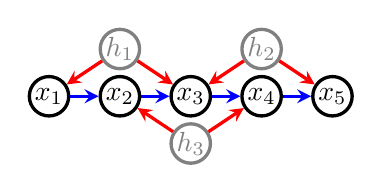
\begin{tikzpicture}[>=stealth, node distance=0.9cm]
    \tikzstyle{format} = [draw, very thick, circle, minimum size=5.0mm,
	inner sep=0pt]

	\begin{scope}
		\path[->, very thick]
			node[format] (x1) {$x_1$}
			node[format, right of=x1] (x2) {$x_2$}
			node[format, right of=x2] (x3) {$x_3$}
			node[format, right of=x3] (x4) {$x_4$}
			node[format, right of=x4] (x5) {$x_5$}

			(x1) edge[blue] (x2)
			(x2) edge[blue] (x3)
			(x3) edge[blue] (x4)
			(x4) edge[blue] (x5)

			node[format, above of=x2, gray, yshift=-0.3cm] (h1) {$h_1$}
			node[format, above of=x4, gray, yshift=-0.3cm] (h2) {$h_2$}
			node[format, below of=x3, gray, yshift=+0.3cm] (h3) {$h_3$}
			
			(h1) edge[red] (x1)
			(h1) edge[red] (x3)
			(h2) edge[red] (x5)
			(h2) edge[red] (x3)

			(h3) edge[red] (x2)
			(h3) edge[red] (x4)

		;
	\end{scope}

\end{tikzpicture}
\end{center}
\caption{ A hidden variable causal DAG.
}
\label{fig:simple}
\end{figure}

Use do-calculus to give an identifying expression for
$p(x_5 \mid \text{do}(x_3))$ in terms of $p(x_1,x_2,x_3,x_4,x_5)$
in a hidden variable causal model in Fig. \ref{fig:simple}.  Note: your expression is not allowed
to refer to $h_1,h_2,h_3$ as those variables are not observed.\\
\textbf{Ans:}\\
$P(X_5 | do(x_3))$\\
$=^p\sum_{x_1}\sum_{x_2}\sum_{x_4}P(X_5, x_1, x_2, x_4|do(x_3))$\\
$=^c\sum_{x_1}\sum_{x_2}\sum_{x_4}P(X_5|x_1, x_2, x_4, do(x_3))P(x_1, x_2, x_4|do(x_3))$\\
$=^c\sum_{x_1}\sum_{x_2}\sum_{x_4}P(X_5|x_1, x_2, x_4, do(x_3))P(x_4|x_1, x_2, do(x_3))P(x_1, x_2|do(x_3))$\\
$=^c\sum_{x_1}\sum_{x_2}\sum_{x_4}P(X_5|x_1, x_2, x_4, do(x_3))P(x_4|x_1, x_2, do(x_3))P(x_2|x_1, do(x_3))P(x_1|do(x_3))$\\
$=^3\sum_{x_1}\sum_{x_2}\sum_{x_4}P(X_5|x_1, x_2, x_4, do(x_3))P(x_4|x_1, x_2, do(x_3))P(x_2|x_1, do(x_3))P(x_1)$\\
%
$=^2\sum_{x_1}\sum_{x_2}\sum_{x_4}P(X_5|x_1, x_2, x_4, do(x_3))P(x_4|x_1, x_2, x_3)P(x_2|x_1, do(x_3))P(x_1)$\\
$=^2\sum_{x_1}\sum_{x_2}\sum_{x_4}P(X_5|x_1, x_2, do(x_4), do(x_3))P(x_4|x_1, x_2, x_3)P(x_2|x_1, do(x_3))P(x_1)$\\
$=^3\sum_{x_1}\sum_{x_2}\sum_{x_4}P(X_5|x_1, x_2, do(x_4))P(x_4|x_1, x_2, x_3)P(x_2|x_1, do(x_3))P(x_1)$\\
$=^{\text{add } x'_3}\sum_{x_1}\sum_{x_2}\sum_{x_4}\sum_{x'_3}P(x_5, x'_3|x_1, x_2, do(x_4))P(x_4|x_1, x_2, x_3)P(x_2|x_1, do(x_3))P(x_1)$\\
$=^c\sum_{x_1}\sum_{x_2}\sum_{x_4}\sum_{x'_3}P(X_5|x'_3, x_1, x_2, do(x_4))P(x'_3|x_1, x_2, do(x_4))P(x_4|x_1, x_2, x_3)P(x_2|x_1, do(x_3))P(x_1)$
$=^2\sum_{x_1}\sum_{x_2}\sum_{x_4}\sum_{x'_3}P(X_5|x'_3, x_1, x_2, x_4)P(x'_3|x_1, x_2, do(x_4))P(x_4|x_1, x_2, x_3)P(x_2|x_1, do(x_3))P(x_1)$
$=^3\sum_{x_1}\sum_{x_2}\sum_{x_4}\sum_{x'_3}P(X_5|x'_3, x_1, x_2, x_4)P(x'_3|x_1, x_2)P(x_4|x_1, x_2, x_3)P(x_2|x_1, do(x_3))P(x_1)$
$=^3\sum_{x_1}\sum_{x_2}\sum_{x_4}\sum_{x'_3}P(X_5|x'_3, x_1, x_2, x_4)P(x'_3|x_1, x_2)P(x_4|x_1, x_2, x_3)P(x_2|x_1)P(x_1)$



\paragraph{2. (10 points) Structure Learning}

We have data on four variables $x_1, x_2, x_3, x_4$, and running a set of
hypothesis tests we learned that the following set of conditional
independences hold in our data:
$(x_2 \ci x_3 \mid x_1)$, $(x_4 \ci x_1 \mid x_2, x_3)$.  Assuming our data was
generated by a DAG model (Bayesian network), give the set of DAGs consistent
with the set of independences we see.  Are there any causal effects with a single outcome (e.g. $p(x_i \mid \text{do}({\bf x}))$, where ${\bf x} = \{ x_j \mid i \neq j \}$) that could be
identified by the same expression, \emph{regardless} of which DAG in the set is
the true DAG?\\
\textbf{Ans:}\\
The correponding DAGs are shown below.
\begin{center}
\includegraphics[scale=0.7]{DAG}
\end{center}
The three DAG graphs above have the same skeleton and the same unshielded collider that is node $X_4$. Therefore, regardless which one is the real graph, they will result in a single outcome by the theorem "Verma and Pearl". They are observational equivalence





\end{document}


